\chapter{Structure from Composite Tasks}
\label{toc:structure_from_composite_tasks}
Prerequisites?
\begin{itemize}
    \item Measureable spaces
    \item Function Spaces
\end{itemize}


\section{Probabilistic Numerics}
\label{toc:probabilistic_numerics}
\begin{figure}[t]
    \centering
    \includestandalone{figures/quantities_of_interest}
    \caption[Quantities of interest]{
        Quantities of interest.
        \label{fig:probabilistic_numerics:quantities_of_interest}
    }
\end{figure}
\begin{definition}[Numerical Method]
    \label{def:probabilistic_numerics:numerical_method}
    Let $\Uc$, $\Yc$ and $\Qc$ be measurable spaces and $Q: \Uc \to \Qc$ a measurable function.
    A \emph{numerical method} $(Y, A)$ for estimation of a quantity of interest $Q$ consists of
    \begin{labeling}{Information operator $Y$\quad}
        \item[Information operator $Y$] A measurable function in $\Uc \to \Yc$;
        \item[Estimation operator $A$] A measurable function in $\Yc \to \Qc$.
    \end{labeling}
\end{definition}

Just like everybody else, we use quadrature as a motivating example to show what quantities of interest are.
We assume $\Uc = \Fun*{C^0}{[a, b]; \Rb}$, the space of continuous real-valued functions on $[a, b]$.
The corresponding quantity of interest space is $\Qc = \Rb$ with the respective values given by the integral
\begin{align}
    Q(u) = \int_a^b u(t) \diff t
\end{align}
We choose $\Yc \subset \Rb^2$ with the information operator
\begin{align}
    Y_{\mat{x}}(u) = \left( \mat{x}, u(\mat{x}) \right)
\end{align}
which evaluates $u$ at the points $\mat{x} \in \Rb^N$ of our choice.
We can freely choose the vector $x_i$, giving rise to different information operators.
Here are a few well-known choices:
\paragraph{Monte Carlo integration}
Here, no explicit assumption about the form of $u$ are made.
\begin{align}
    \mat{x}
     & \sim \Uniform{[a, b]^N}
     & \Fun*{A_{\text{MC}}}{(\mat{x}, u(\mat{x})}
     & = \frac{1}{N} \sum_n u(x_n)
\end{align}

\paragraph{Trapezodial Rule}
The trapezodial rule approximates a function via a piecewise linear surrogate which is then integrated.
\begin{align}
    \mat{x}
     & = a + \frac{b - a}{N - 1} \cdot (0, 1, \cdots, N - 1)
     & \Fun*{A_{\text{TZ}}}{(\mat{x}, u(\mat{x})}
     & = \sum_{n=0}^{N - 1} \frac{b - a}{2} \left( u(x_{n-1}) + u(x_n) \right)
\end{align}

Note that all of these choices up to here are completely arbitrary, so none of those methods need to be particularly good.
They can, of cause, be motivated quite well.
We will show now how this motivation can be put in a probabilistic context.


\begin{figure}[t]
    \centering
    \includestandalone{figures/probabilistic_numerics}
    \caption[Probabilistic Numerics]{
        Probabilistic Numerics.
        \label{fig:probabilistic_numerics:probabilistic_numerics}
    }
\end{figure}
\begin{definition}[Probabilistic Numerical Method]
    \label{def:probabilistic_numerics:probabilistic_numerical_method}
    Let $\Uc$, $\Yc$ and $\Qc$ be measurable spaces and let $Q: \Uc \to \Qc$ be a measurable function.
    A \emph{probabilistic numerical method} $(Y, B)$ for estimation of a quantity of interest $Q$ consists of
    \begin{labeling}{Belief update operator $B$\quad}
        \item[Information operator $Y$] A measurable function in $\Uc \to \Yc$;
        \item[Belief update operator $B$] A measurable function in $\Probs{\Uc} \times \Yc \to \Probs{\Qc}$.
    \end{labeling}
\end{definition}

Explain Monte Carlo here?

\begin{definition}[Disintegration]
    Let $\Uc^y = \Set{u \in \Uc \with Y(u) = y}$.
    For $p \in \Probs{\Uc}$, a collection $\Set{p^y}_{y \in \Yc} \subset \Probs{\Uc}$ is a \emph{disintegration of $p$} with respect to a measurable $Y: \Uc \to \Yc$ if
    \begin{labeling}{Concentration\quad}
        \item[Concentration] $\Fun*{p^y}{\Uc \setminus \Uc^y} = 0$ for $Y_\#p$-almost all $y \in \Yc$;
        \item[Measurability] $y \mapsto p^y(f)$ is measurable;
        \item[Conditioning] $p(f) = \int p^y(f) Y_\#p(\diff y)$;
    \end{labeling}
    for each measurable $f : \Uc \to [0, \infty)$.
\end{definition}
This is an extension to conditionings of Random variables to the case where $\Uc^y$ is a null set.
Existence of disintegrations is guaranteed under weak conditions.

\begin{definition}[Bayesian Probabilistic Numerical Method]
    \label{def:probabilistic_numerics:bayesian_probabilistic_numerical_method}
    A probabilistic numerical method $M = (Y, B)$ is called \emph{Bayesian} for a quantity of interest $Q$ if for all $p \in \Probs{\Uc}$ and for $Y_\#p$-almost-all $y \in \Yc$
    \begin{align}
        \Fun*{B}{p, y} = Q_\#p^y.
    \end{align}
\end{definition}

Explain Trapezodial Rule here.
\begin{theorem}[The good theorem.]
    Everything is true.
\end{theorem}


\section{Bayesian Optimization}
\label{toc:bayesian_optimization}
Bayesian optimization (BO) methods often rely on the assumption that the objective function is well-behaved, but in practice, this is seldom true for real-world objectives even if noise-free observations can be collected.
Common approaches, which try to model the objective as precisely as possible, often fail to make progress by spending too many evaluations modeling irrelevant details.
We address this issue by proposing surrogate models that focus on the well-behaved structure in the objective function, which is informative for search, while ignoring detrimental structure that is challenging to model from few observations.
First, we demonstrate that surrogate models with appropriate noise distributions can absorb challenging structures in the objective function by treating them as irreducible uncertainty.
Secondly, we show that a latent Gaussian process is an excellent surrogate for this purpose, comparing with Gaussian processes with standard noise distributions.
We perform numerous experiments on a range of BO benchmarks and find that our approach improves reliability and performance when faced with challenging objective functions.

\subsection{Introduction}
\label{toc:bayesian_optimization:introduction}
\begin{figure}[t]
    \centering
    \raisebox{-0.5\height}{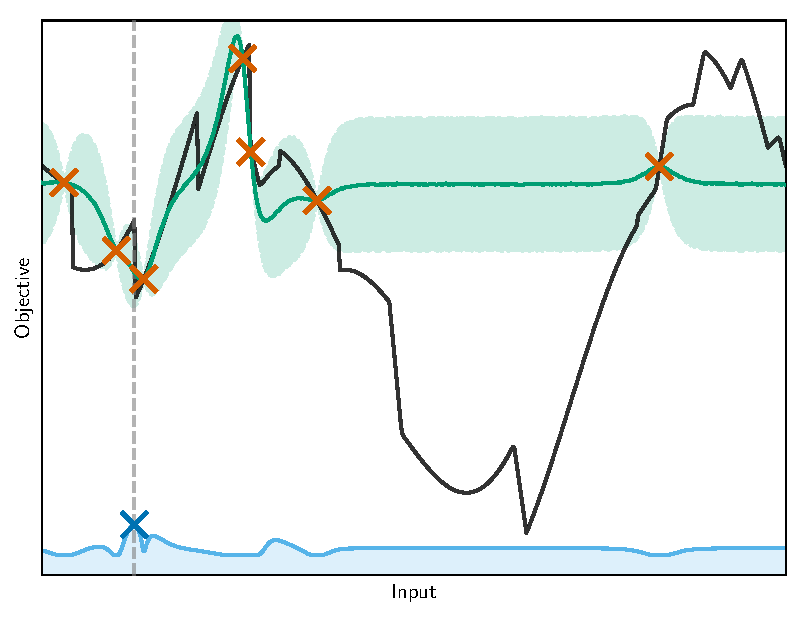
\includegraphics[trim=15 15 0 0, clip, width=0.25\textwidth]{robust_bo_erik/illustrative_figure/gp.pdf}}
    \raisebox{-0.5\height}{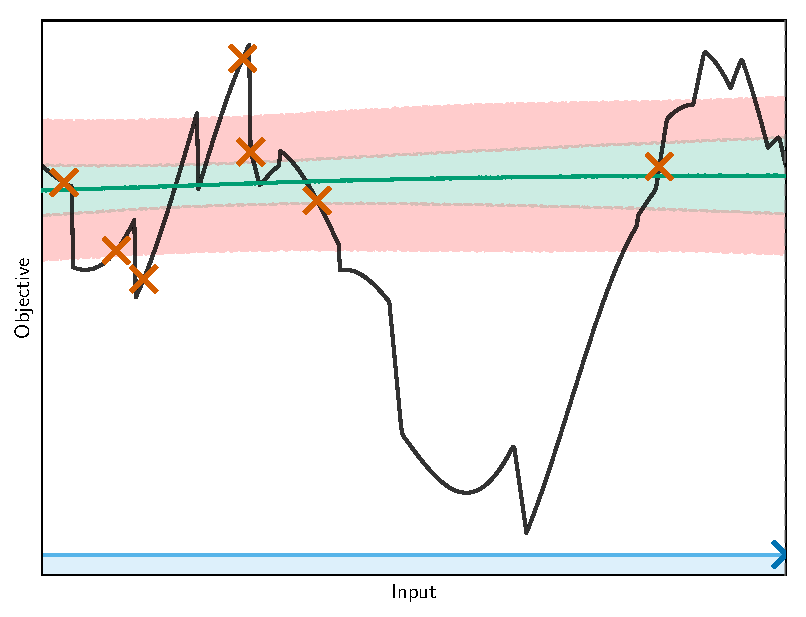
\includegraphics[trim=15 15 0 0, clip, width=0.25\textwidth]{robust_bo_erik/illustrative_figure/homo_gp.pdf}}
    \raisebox{-0.5\height}{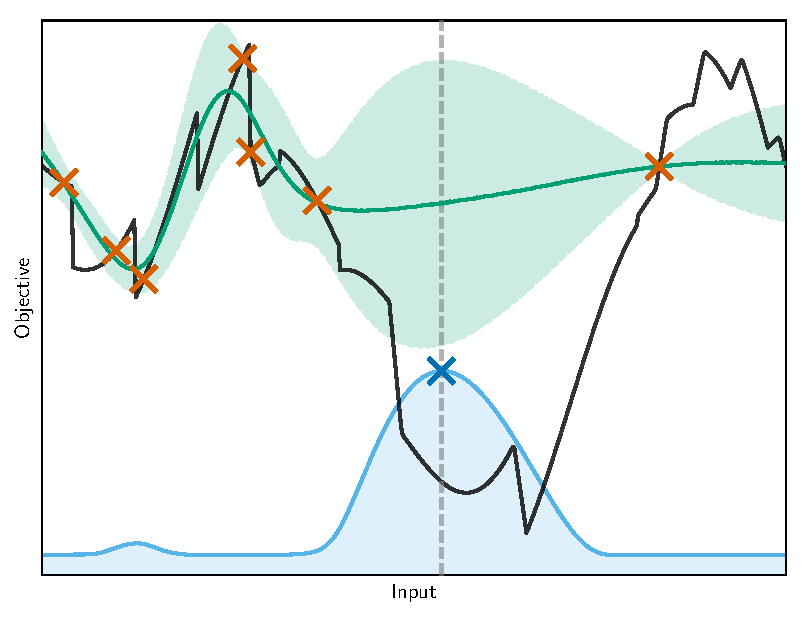
\includegraphics[trim=15 15 0 0, clip, width=0.25\textwidth]{robust_bo_erik/illustrative_figure/modulating_lgp.pdf}}
    \raisebox{-0.45\height}{{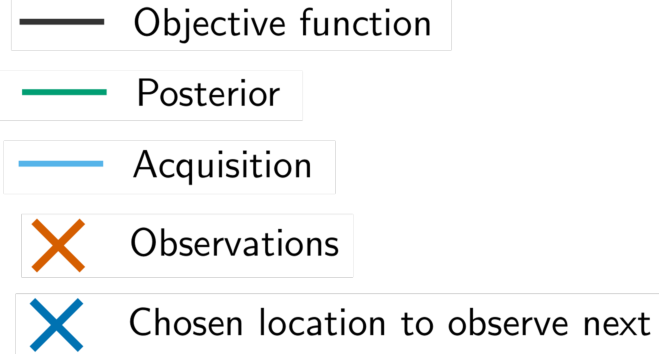
\includegraphics[width=0.20\textwidth]{robust_bo_erik/illustrative_figure/legend_compact.pdf}}}
    \caption{
        \label{fig:bayesian_optimization:posterior}
        An illustrative example of the posterior surrogate function density obtained given observations of a 1D nonsmooth function
        using a noise-free GP, a GP with homoscedastic Gaussian noise, and using a LGP model.
        The posterior belief for the noise-free and homoscedastic GP surrogates results in the EI acquisition function,
        shown in blue,
        making poorly informed decisions for the next query.
        In contrast, the LGP using our proposed setup is able to reduce the influence of the rapid oscillations that do not match the GP prior by explaining part of the variation using the latent input.
        As a result, the acquisition function can utilize a confidently discovered global trend to increase the efficiency of the search.
        In this example, $\sigma_h$ is set to $\frac{1}{50}$ of the domain range to allow ignorance of oscillations at that scale.
    }
\end{figure}
Bayesian optimization (BO)~\parencite{snoek_practical_2012} is a method for finding the optimum of functions that are unknown and expensive to evaluate.
By fitting a surrogate model to the samples of an unknown objective, the BO procedure iteratively picks the new samples of the objective believed to be the most informative about where the optimum is located.

Model misspecification has significant negative implications for any machine learning tasks.
This is especially true for sequential decision making tasks such as BO, where the model is used not only to locate the optimum based on the collected data but also to decide where to collect data for future decisions.
If the surrogate model is misspecified, it is likely to acquire samples that are less informative about the optimum, which will lead to a less efficient optimization.
Therefore the quality of the surrogate model is essential to achieve both efficient and reliable results.

Many works have been done towards avoiding model misspecification in the surrogate model for BO, such as handling non-stationary objective functions with warpings~\parencite{snoek_input_2014}, tree-structured dependencies in the search space~\parencite{jenatton_bayesian_2017}, and searching the optimum from piecewise comparisons~\parencite{gonzalez_preferential_2017}.
Comparing with the Gaussian process (GP) regression model in the standard BO setting, these methods avoid model misspecification in real-world problems by using more sophisticated surrogate models that are suitable for the corresponding problems.
Bayesian inference with more sophisticated surrogate models will often require additional data to reduce uncertainty and confirm beliefs, because it considers more possibilities.
Importantly the ultimate goal of BO is to find the optimum, not to model the unknown objective as precisely as possible.
In practice, this means that using a surrogate with high complexity might perform worse compared to a simpler class
even if the former contains the true objective function.

Instead of building a complex surrogate model with minimal model misspecification,
we propose an alternative approach which allows trading off accuracy in modeling the objective with efficiency of capturing informative structures from small amounts of data.
For example, we observe that structures such as local oscillations and discontinuities are less important to capture for the purposes of BO.
Such details often require a lot of data to be closely captured in a surrogate model but do not help the search for the optimum,
unless the search reaches the last stage of pinpointing the exact location of the optimum.
To ignore these details, we associate an independent random \emph{input} variable with every evaluation of the unknown function.
As the random variables associated with new evaluations are conditionally independent of the posterior random variables associated with observed data given the function,
this is referred to as \emph{irreducible uncertainty}.
Such variables are similar to the noise variables in regression models, which are used to capture measurement noise and the data variance that cannot be attributed to the input variables.
In contrast to noise variables for noisy outcomes,
where there is irreducible uncertainty about the data, there is now irreducible uncertainty in the model of the function.

We propose to use the surrogate models that are specified over well-behaved approximations of the objectives,
which can be more useful for the search of the optimum (see \cref{fig:bayesian_optimization:posterior}), augmented with flexible ``noise" distributions.
We will demonstrate that, using the same function approximation, a surrogate model with a more flexible noise distribution is more robust against challenging structures.
In this paper we focus on noise-free objectives with complicated, oscillatory or discontinuous structures.
In particular, we propose to use a Latent Gaussian process (LGP)~\parencite{pfingsten_nonstationary_2006,wang_gaussian_2012,yousefi_unsupervised_2016,bodin_latent_2017} as the surrogate model due to its flexible noise distribution and show that it outperforms the surrogate models with less flexible noise distributions such as GPs with additive noise.
LGP allows us to disentangle the complicated structures a GP surrogate struggles to model while highlighting important structures.

Our main contributions are:
\begin{itemize}
    \item We propose to address challenging objective functions for BO by using a distribution in the surrogate model to explain structure that is challenging to model with few observations.
    \item We propose to use latent Gaussian processes (LGP) as surrogate models, which support non-stationary and non-Gaussian residuals.
    \item With experiments on multiple BO benchmarks, we show that our method significantly outperforms existing approaches.
\end{itemize}

\subsection{Modulating Surrogates}
\label{toc:bayesian_optimization:modulated_objectives}

Let $f : \Xc \to \Rb$ be an unknown, noise-free objective function defined on a bounded subset $\Xc \subset \Rb^Q$.
The goal of BO is to solve the global optimization problem of finding
\begin{equation}
    \mat{x}_{\text{min}} = \argmin_{\mat{x} \in \Xc} f(\mat{x}).
\end{equation}
In real world problems,
the objective function is often not a well-behaved function and a suitable model is difficult to specify.
Instead of applying an automated model selection method~\parencite{malkomes_automating_2018},
we propose to model only the essential structure of the objective function that is well-behaved and leave the rest of the function details to be absorbed in a noise distribution.

We consider the family of objective functions $f$ that can be represented as a composition of a well-behaved function and another arbitrary, latent function capturing the challenging details, i.e.
\begin{equation}
    \label{eq:bayesian_optimization:well_behaved}
    f(\mat{x}) := g(\mat{x}, \mat{h}), \quad \mat{h}:=h(\mat{x}),
\end{equation}
where $g$ is a well-behaved function that can be nicely modeled by a surrogate model of choice,
which is a Gaussian process (GP) in this paper,
and the vector-valued function $h(\mat{x})$ encodes the structures which the surrogate model struggles to capture.
In general this composition allows for complicated interactions between $\mat{x}$ and $\mat{h}$, producing complicated realizations of the function
which is observed through data.
A simple, special case of such a function composition is additive structure
\footnote{Note that in the additive case, $h(\mat{x})$ must match the output in shape, i.e.~be one-dimensional.},
i.e.\ $f(\mat{x}) = g(\mat{x}) + h(\mat{x})$.
%which has been exploited for BO~\parencite{gardner_discovering_2017, mutny2018efficient}.

Instead of modeling $h(\mat{x})$ as part of the surrogate model,
we propose to \textit{ignore} the structure of the objective function in $h(\mat{x})$ by replacing $h(\mat{x})$ with a random variable $\mat{h}$ per data point.
The random variables $\mat{h}$ for different data points  are independent among each other.
The objective function becomes a function of two variables $g(\mat{x}, \mat{h})$,
in which $\mat{h}$ is a random variable which explain the data variance that cannot be explained by $\mat{x}$.
In this paper, we use a normal distribution for the prior of $\mat{h}$, $\mat{h} \sim \mathcal{N}(0,  \mathbb{I})$.
Note that, although the distribution of $h(\mat{x})$ induced by the data distribution for $\mat{x}$ may not be zero-mean and unit-variance, it is easy to reformulate it as a linear transformation of a normal distribution with zero-mean and unit-variance and the resulting linear transformation can be absorbed into the function $g$.
For further details on the definition, see the supplement.

With the above formulation, a BO method can be developed by constructing a surrogate model for the well-behaved function $g$.
At each step of the BO optimization, a set of input and output pairs of the objective function has been collected, denoted as $\mat{X} = (\mat{x}_1, \ldots, \mat{x}_N)^\top$ and $\mat{F} = (\mat{f}_1, \ldots, \mat{f}_N)^\top$.
The output $\mat{F}$ denotes the noise-free observations of the objective function, which is the assumption in this paper but is straight-forward to extend to the case of noisy observations.
The Bayesian inference of the surrogate model aims at inferring the posterior distribution
\begin{equation}
    \Prob{ \mat{H}, \mat{\theta} \given \mat{X}, \mat{F}}  \propto \Prob{\mat{F} \given \mat{X}, \mat{H}, \mat{\theta} }\Prob{\mat{H}}  \Prob{\mat{\theta}}
\end{equation}
where $\mat{\theta}$ are the hyper parameters of the surrogate model and $\mat{H} = (\mat{h}_1, \ldots, \mat{h}_N)^\top$ is the concatenation of the noise variables of individual data points.
The location of the next evaluation is determined according to an acquisition function,
which uses the predictive distribution $\Prob{\mat{f}_* \given \mat{x}_*,  \mat{X}, \mat{F}}$ of the surrogate model,
where $\mat{x}_*$ is the input of the prediction and $\mat{f}_*$ is the noise-free observation at the location $\mat{x}_*$.
The standard formulation of such a predictive distribution is
\begin{align}
    \begin{split}
        \MoveEqLeft\Prob{\mat{f}_* \given \mat{x}_*,  \mat{X}, \mat{F}} =
        \int \Prob{\mat{f}_* \given \mat{x}_*, \mat{h}_*, \mat{X}, \mat{F},\mat{H}, \mat{\theta}}\\
        &\qquad\Prob{\mat{H}, \mat{\theta} \given \mat{X}, \mat{F}} \Prob{\mat{h}_*} \diff{\mat{H}}\diff{\mat{\theta}}\diff{\mat{h}_*},
    \end{split}
\end{align}
where $\mat{h}_*$ is the noise variable corresponding to the input $\mat{x}_*$.
The above distribution of $\mat{f}_*$ contains the uncertainty that comes from the randomness of $\mat{h}_*$.
This is \textit{undesirable} because the uncertainty due to $\mat{h}_*$ is irreducible uncertainty (see \cref{toc:bayesian_optimization:introduction}), which is not helpful in terms of finding the optimum of the objective function with respect to $\mat{x}$.
A failure mode is that the BO search gets stuck by repeatedly collecting evaluations at the location where the uncertainty due to $\mat{h}_*$ is high as this uncertainty cannot be reduced.
In some cases, including such irreducible uncertainty can completely mislead the search~\parencite{gonzalez_preferential_2017}.
We propose to remove the uncertainty contributed by $\mat{h}_*$ by collapsing the prior distribution of $\mat{h}_*$ into a Dirac delta distribution, $\hat{p}(\mat{h}_*) = \delta(\mat{h}_*)$.
With this modified prior distribution, the predictive distribution of $\mat{f}_*$ can be obtained without the uncertainty from $\mat{h}_*$,
\begin{align}
    \begin{split}
        \MoveEqLeft\hProb{\mat{f}_* \given \mat{x}_*,  \mat{X}, \mat{F}} =
        \int \Prob{\mat{f}_* \given \mat{x}_*,\mat{h}_*,  \mat{X}, \mat{F},\mat{H}, \mat{\theta}} \\
        &\qquad\qquad\Prob{\mat{H}, \mat{\theta} \given \mat{X}, \mat{F}} \hProb{\mat{h}_*} \diff{\mat{\theta}}\diff{\mat{H}}\diff{\mat{h}_*} \\
        &= \int \Prob{\mat{f}_* \given \mat{x}_*,\mat{h}_*=\mat{0},  \mat{X}, \mat{F},\mat{H}, \mat{\theta}} \\
        &\qquad\qquad\Prob{\mat{H}, \mat{\theta} \given \mat{X}, \mat{F}} \diff{\mat{\theta}}\diff{\mat{H}}.
    \end{split}
\end{align}
In the supplement we provide an example illustrating the effect of including such irreducible uncertainty,
together with further details.

With the above predictive distribution, the new expectation of the acquisition function can be derived as
\begin{align}
    \begin{split}
        \label{eq:bayesian_optimization:utility}
        \MoveEqLeft[1]\alpha(\mat{x}_\ast) =
        \int
        \mathbb{U}(\mat{f}_\ast, \mat{x}_\ast, \mat{X}, \mat{F}) \hat{p}(\mat{f}_\ast | \mat{x}_\ast, \mat{X}, \mat{F}) \diff{\mat{f}_\ast},
    \end{split}
\end{align}
where the acquisition function of choice is denoted $\mathbb{U}$.
Note that the predictive distribution due to the marginalization over $\mat{H}$ and $\mat{\theta}$ generally has a complicated form
and that the above integral often requires approximate methods.

\subsection{Latent GP surrogates and other choices}
\label{toc:bayesian_optimization:latent_gp_surrogate}

\begin{figure}[t]
    \centering
    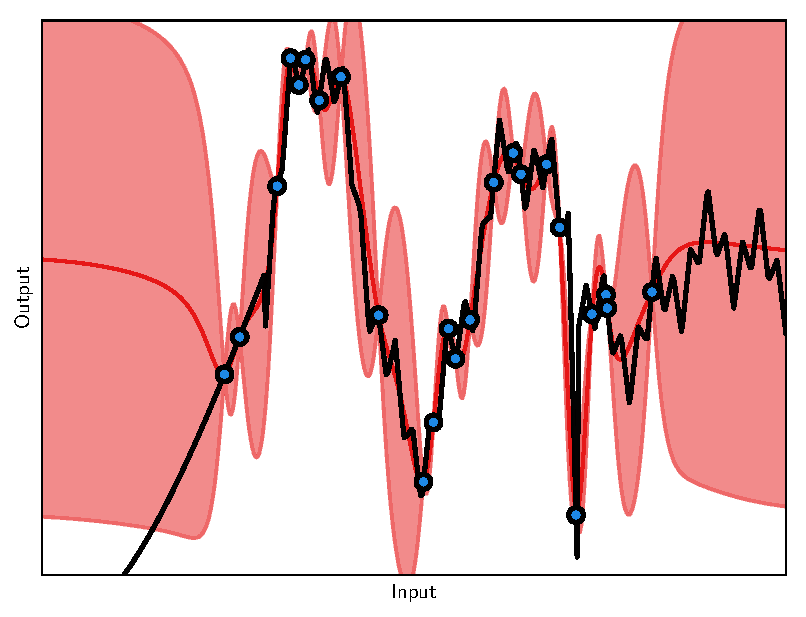
\includegraphics[trim={0.5cm 0.5cm 0 0},clip, width=0.19\textwidth]{robust_bo_erik/z_varying_eps_1_div_10000000000.pdf}
    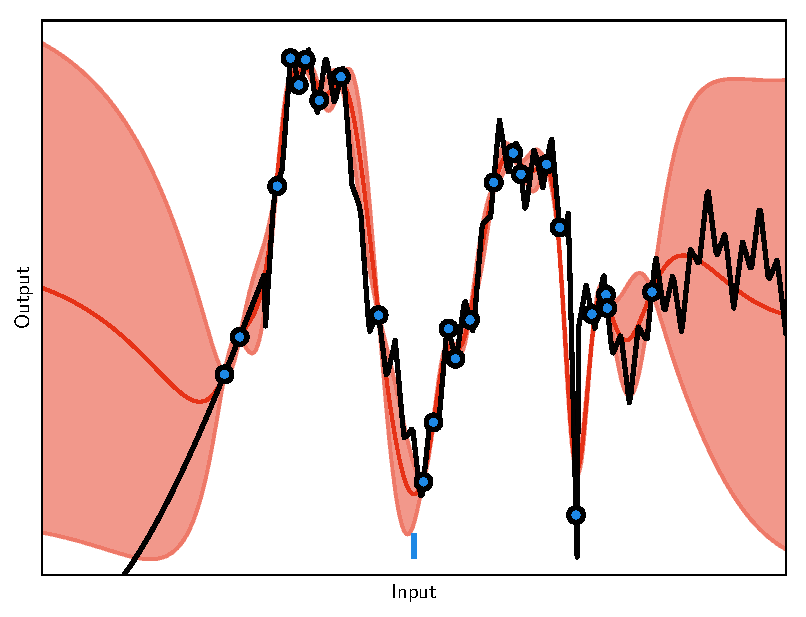
\includegraphics[trim={0.5cm 0.5cm 0 0},clip, width=0.19\textwidth]{robust_bo_erik/z_varying_eps_1_div_1000.pdf}
    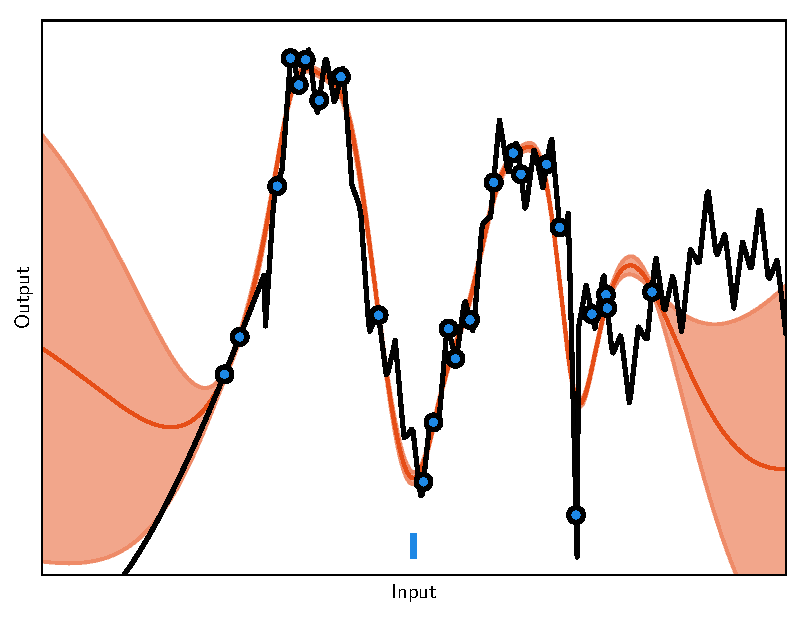
\includegraphics[trim={0.5cm 0.5cm 0 0},clip, width=0.19\textwidth]{robust_bo_erik/z_varying_eps_1_div_500.pdf}
    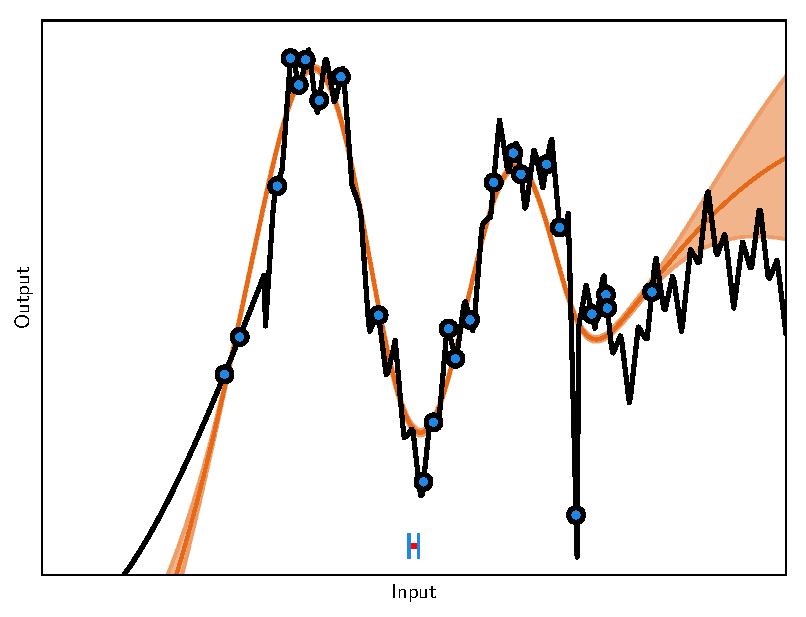
\includegraphics[trim={0.5cm 0.5cm 0 0},clip, width=0.19\textwidth]{robust_bo_erik/z_varying_eps_1_div_100.pdf}
    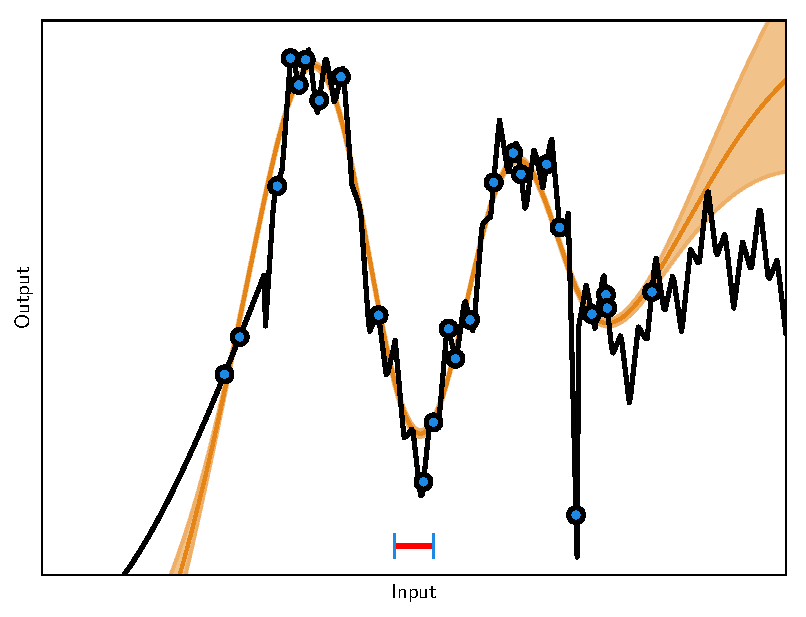
\includegraphics[trim={0.5cm 0.5cm 0 0},clip, width=0.19\textwidth]{robust_bo_erik/z_varying_eps_1_div_20.pdf}\\
    \hspace{-0.01cm}
    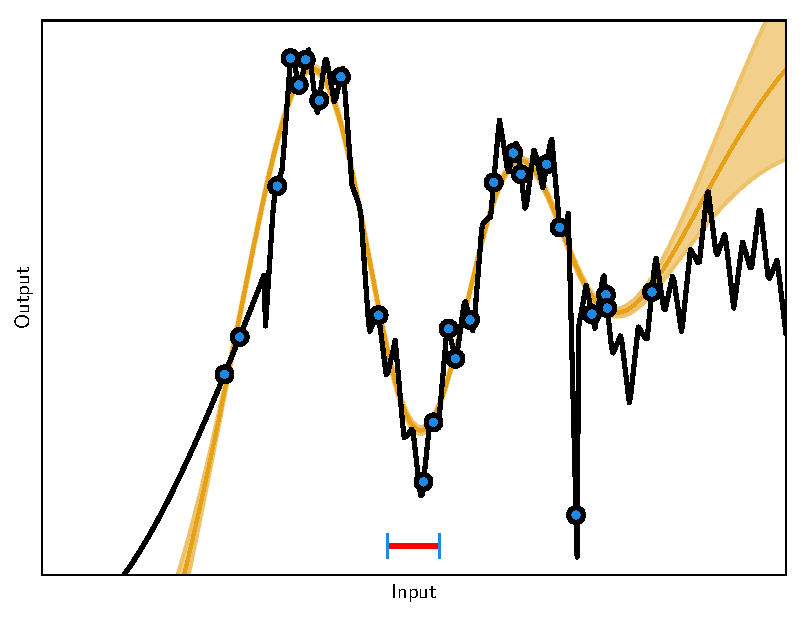
\includegraphics[trim={0.5cm 0.5cm 0 0},clip, width=0.19\textwidth]{robust_bo_erik/z_varying_eps_1_div_15.pdf}
    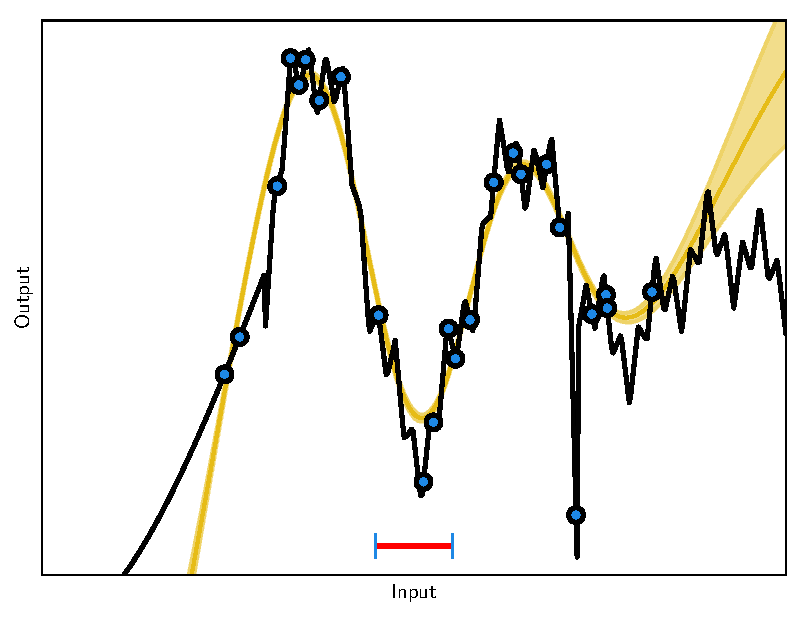
\includegraphics[trim={0.5cm 0.5cm 0 0},clip, width=0.19\textwidth]{robust_bo_erik/z_varying_eps_1_div_10.pdf}
    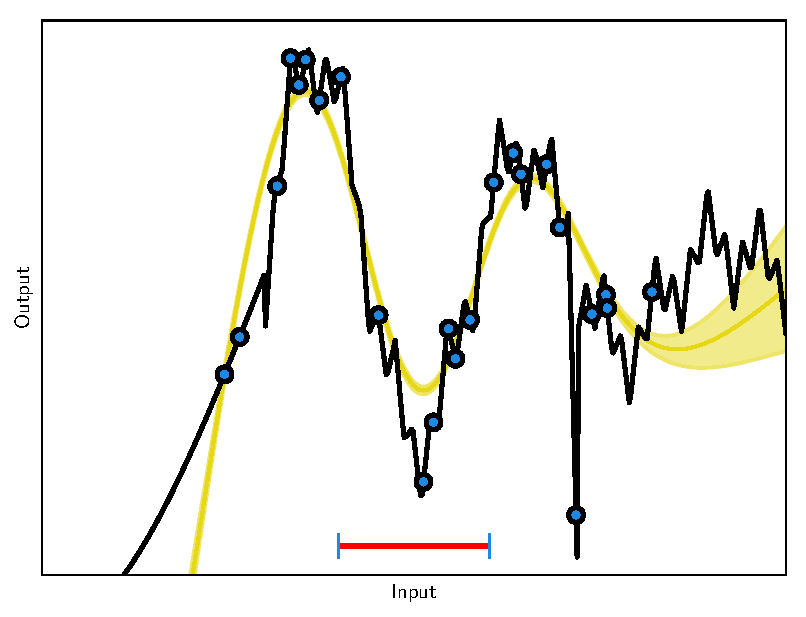
\includegraphics[trim={0.5cm 0.5cm 0 0},clip, width=0.19\textwidth]{robust_bo_erik/z_varying_eps_1_div_5.pdf}
    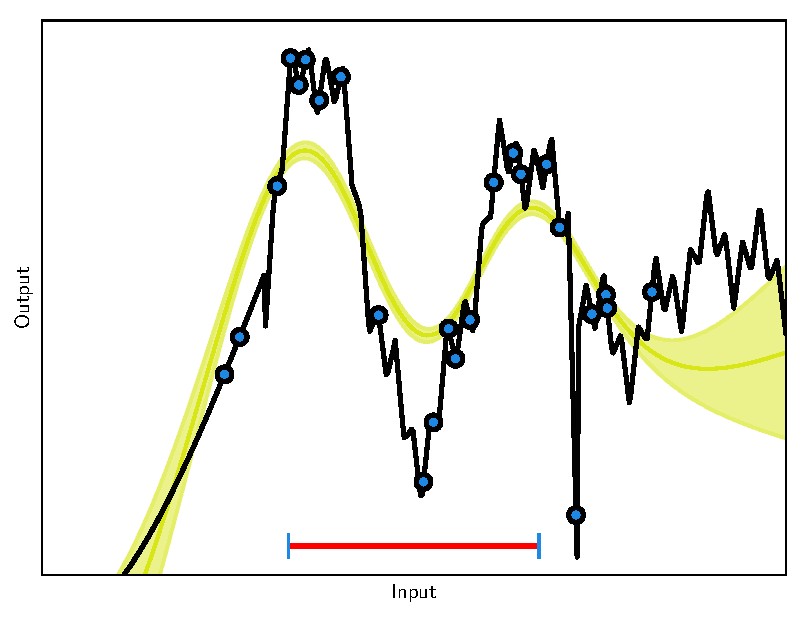
\includegraphics[trim={0.5cm 0.5cm 0 0},clip, width=0.19\textwidth]{robust_bo_erik/z_varying_eps_1_div_3.pdf}
    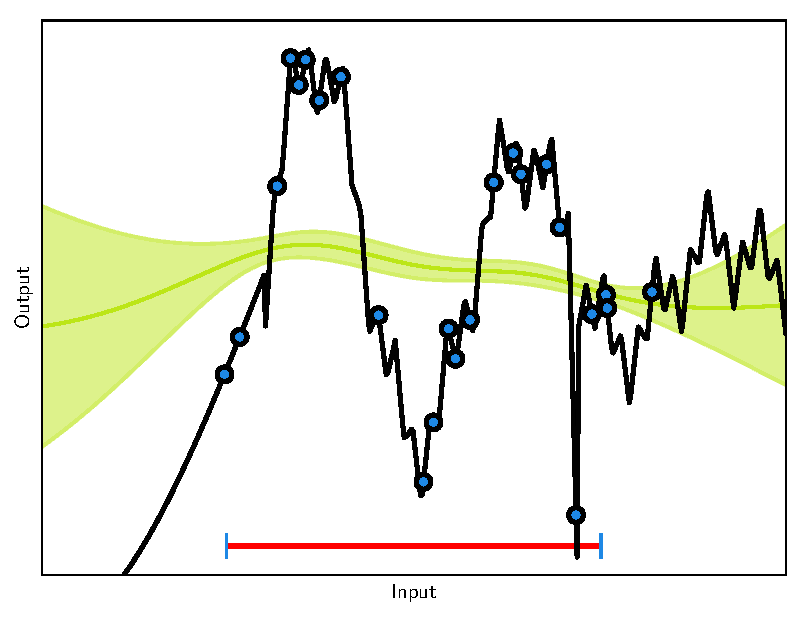
\includegraphics[trim={0.5cm 0.5cm 0 0},clip, width=0.19\textwidth]{robust_bo_erik/z_varying_eps_1_div_2.pdf}
    \caption{
        \label{fig:bayesian_optimization:varying_z_sigma}
        Input-related invariance.
        Each plot is showing the resulting modulated function posterior using the LGP model and setting $\sigma_h$ in $p(\mat{h})$ to a size corresponding to the
        red line at the bottom of respective plot.
        The posterior is shown with mean and two standard deviations.
        The true function is shown in black.
        Note how the value of the prior $\sigma_h$ sets the scale in relation to $\Xc$ on how much detail is ignored.
        A connection can be made to low-pass filtering of higher frequencies, but where the filter varies between observations as of the posterior and where each filter is implicitly determined
        by fit to the function prior.
    }
\end{figure}

In the previous subsection we presented the BO formulation.
We will now proceed to implement the formulation, and address the choice of surrogate model for the function \cref{eq:bayesian_optimization:well_behaved}.

\textbf{Additive noise model.}
As briefly mentioned in the previous subsection, a simple case of the composition \cref{eq:bayesian_optimization:well_behaved} is an additive structure, $f(\mat{x}) = g(\mat{x})+h(\mat{x})$.
Following the process of replacing $h(\mat{x})$ with the random variable $\mat{h}$, the resulting surrogate model of the objective function is
\begin{equation}
    f(\mat{x}) = g(\mat{x}) + h, \quad h \sim \mathcal{N}(0, \sigma(\mat{x})^2),
\end{equation}
where the variance of $h$ is assumed to be $\sigma^2$ in order to adapt to the value range of $f$.
With a GP surrogate model for $g$, the above model recovers the GP regression model with the Gaussian likelihood.
%The major difference in our approach is that we infer the noise variance $\sigma^2$ even though the objective function is noise-free.

A typical choice in the above model is to assume $\sigma^2$ to be constant, leading to a homoscedastic model.
A limitation of noise variances being the same across all the datapoints is that it limits the capability of the model in terms of absorbing irregular variance.
A straight-forward extension of the above model is the GP with heteroscedastic noise, in which the noise variance $\sigma^2$ is allowed to be different among data points \parencite{goldberg_regression_1998,lazaro-gredilla_variational_2011}.
Another choice could be specifying a GP prior for $h(\mat{x})$ and thus recover an additive GP model for $f$~\parencite{bernardo_regression_1998,duvenaud_additive_2011}.
Other available choices for an additive noise model include Student's t-distribution~\parencite{jylanki_robust_2011}, Laplace~\parencite{kuss_gaussian_2006} or
mixture of Gaussian likelihoods as~\parencite{kuss_gaussian_2006, stegle_gaussian_2008, naish-guzman_robust_2008} where~\parencite{naish-guzman_robust_2008} considers the heteroscedastic case.

\textbf{Latent Gaussian process.}
A major limitation of the additive noise models in general is the inability to capture the interaction between the input $\mat{x}$ and the noise $\mat{h}$.
Another choice that produces a more flexible noise distribution is to introduce additive noise in the \emph{input} of a GP~\parencite{mchutchon_gaussian_2011,girard_gaussian_2003,girard_approximate_2004}.
This would correspond to the case of $f(\mat{x}) = g(\mat{x} + \mat{h})$.
A further more general case of the proposed methodology is to allow non-linear interactions between the random variable $\mat{h}$ and $\mat{x}$.
This can be formulated as
\begin{equation}
    f(\mat{x}) = g(\mat{x}, \mat{h}),\quad g \sim \mathcal{GP},\quad \mat{h} \sim \mathcal{N}(0, \mathbb{I}). \label{eqn:bayesian_optimization:lgp}
\end{equation}
This formulation aligns with the general assumptions proposed in the previous subsection.
In particular, the well-behaved function $g$ is assumed to follow a GP prior distribution,
and the random variable derived from the challenging details of the objective function $\mat{h}$ feeds directly into the GP surrogate model.
This allows for an arbitrary interaction between $\mat{h}$ and $\mat{x}$, as specified by the covariance function.
The introduction of the random variable $\mat{h}$ in the input results in a flexible noise distribution, as the GP model can warp the normal distribution of $\mat{h}$ into a sophisticated distribution and allow non-linear interactions between $\mat{h}$ and $\mat{x}$.
%
This GP model in \cref{eqn:bayesian_optimization:lgp} is also known as a latent Gaussian process (LGP)~\parencite{pfingsten_nonstationary_2006,wang_gaussian_2012,yousefi_unsupervised_2016,bodin_latent_2017}, which is developed for regression with heteroscedastic noise and non-Gaussian residuals.
The non-Gaussian marginals arise as a consequence of the latent covariates and their nonlinear transformation through the covariance function.

%Now we will show how we can interpret and parameterize such a model to implicitly encode beliefs about function structures that are informative for the search of the optimum.

\paragraph{Function modulation via $\Zc$}
If we assume a stationary kernel over the product space $\Xc \times \Zc$, a constant $\mat{h}_n$ for all observations can be interpreted as the $\Zc$ subspace having no influence.
This is due to the stationary property of the kernel, where covariances are determined only by the distances between points.

With everything else held constant, if an observation is moved away from other observations in the $\Zc$ space, the covariances between that observation and the others are reduced.
Similarly, if the length scale in $\Xc$-direction is shortened, the covariances between that observation and the others can be equally reduced, but that also reduces the covariances between \emph{all other} observations due to the global influence of the hyperparameter.

Structures in the data could be explained solely by reducing the $\Xc$-direction length scale adequately.
In that case, evaluating the posterior at $\mat{h}_\ast = \mat{0}$ would yield exactly the posterior of a standard GP.
Conversely, structures could be explained solely as observations being adequately far from each other in the $\Zc$ space while maintaining a longer $\Xc$ length scale.
Evaluating the posterior at $\mat{h}_\ast = \mat{0}$ then yields a posterior that is both influenced by the longer length scale and which has lower covariances with the data, effectively producing a posterior over smoother functions.
If the posterior inputs $\mat{H}$ are sufficiently far away with respect to the $\Zc$-direction length scale,
all data variation will be captured in $\Zc$ and the posterior of the function at $\mat{h}_\ast = \mat{0}$ will in effect ignore the data.

The posterior weighting over this range of solutions is determined by the trade-off between the GP function prior and the prior of the latent inputs.
As such, by controlling this trade-off, we can control properties of structures to be ignored and the ones to be used for search (see \cref{fig:bayesian_optimization:varying_z_sigma}).
Important to note is that the mentioned data ignorance effect affects \emph{individual} data points via the posterior of the corresponding latent input $\mat{h}_n$,
which is influenced by the local and global fit of the function prior.

\paragraph{Reparameterization of LGP for ease of specifying the modulation prior}
In a BO setting, some prior knowledge about what constitutes a significant change in the input space is often available.
We would like to specify a joint prior of the GP and the latent inputs to ignore structures at the appropriate scale.
In order to do this, we (re)-parametererise it in the following way.
We set the lengthscale in the $\Zc$-direction to be the same as in the $\Xc$-direction and parameterize the latent input prior as $\mathcal{N}(\mat{h}_n|\mat{0}, \sigma_h^2\mathbb{I})$ instead of a unit Gaussian.
There is an equivalence between parameterizing $\sigma_h$ or setting this trade-off via a separate lengthscale for $\Zc$ as in~\parencite{wang_gaussian_2012}.
However, by using the above parameterization there is a direct correspondence in covariance reduction from moving an observation in $\Zc$ as in $\Xc$, and the prior for the latent inputs can be interpreted as a prior over the coarseness of the function we wish to exploit for search.
As such, intuitions about the scale in $\Xc$ directly translate into the parameterization of the prior.
See \cref{fig:bayesian_optimization:varying_z_sigma} for a visualization of how changing $\sigma_h$ in the prior affects the modulated function posterior.
To make the $\sigma_h$ parameterization relevant across input sizes and dimensionalities,
we rescale the input domain $\Xc$ to be a unit hyper-cube and set $\sigma_h$ proportionally to the length of the diagonal of the domain $\sqrt{Q}$ (where $Q$ is the number of dimensions).

\textbf{Posterior inference and acquisition calculation.}
In BO we assume that $N$ pairs of inputs and outputs $\mat{X} = (\mat{x}_1, \ldots, \mat{x}_N)^\top$ and $\mat{F} = (\mat{f}_1, \ldots, \mat{f}_N)^\top$ have been collected.
To suggest the location for the next evaluation, we first need to infer the posterior distribution of the latent variables, which are $\mat{H}$ and $\mat{\theta}$ in LGP, and then search for the maximum of the acquisition function $\alpha(\mat{x})$.

Given the observed data, the probabilistic model of LGP is formulated as
\begin{align}
    \begin{split}
        \Prob{\mat{F} \given \mat{X}, \mat{H}, \mat{\theta}} = \mathcal{N}(\mat{F} | \mat{0}, \mat{K}),\\
        \Prob{\mat{H}} = \prod_{n=1}^N \mathcal{N}(\mat{h}_n | \mat{0}, \sigma_h^2\mathbb{I}),
    \end{split}
\end{align}
where $\mat{K}$ is the covariance matrix computed using a chosen kernel function $k(\cdot, \cdot)$ over the set of data points $\{\bar{\mat{x}}_n\}_{n=1}^N$, and $\bar{\mat{x}}_n$ is the concatenation of two vectors $(\mat{x}_n^\top, \mat{h}_n^\top)^\top$.
Because $\mat{h}_n^\top$ enters the kernel function non-linearly, it is clear that the posterior distribution $\Prob{\mat{H}, \mat{\theta} \given \mat{F}, \mat{X}}$ is intractable.
To ensure the quality of the acquisition function, usually, BO methods draw posterior samples of latent variables via Markov Chain Monte Carlo (MCMC) methods such as slice sampling~\parencite{snoek_practical_2012} or Hamiltonian Monte Carlo~\parencite{duane_hybrid_1987}.
We follow this practice and provide details in the supplement.

With the approximate posterior samples $\{\mat{H}_i, \mat{\theta}_i\}_{i=1}^M$, we approximate the acquisition function with LGP in \cref{eq:bayesian_optimization:utility} with Monte Carlo samples,
\begin{align}
    \alpha(\mat{x}_\ast) & \approx
    \frac{1}{M}\sum_{i=1}^M \hat{\alpha}(\mat{x}_*, \mat{H}_i, \mat{\theta}_i),
\end{align}
where $\hat{\alpha}(\mat{x}_*, \mat{H}_i, \mat{\theta}_i)$ is the acquisition function given the latent variables of LGP, which is closed-form for common acquisition functions such as expected improvement (EI) and upper confidence bound (UCB).

\begin{figure}[t]
    \centering
    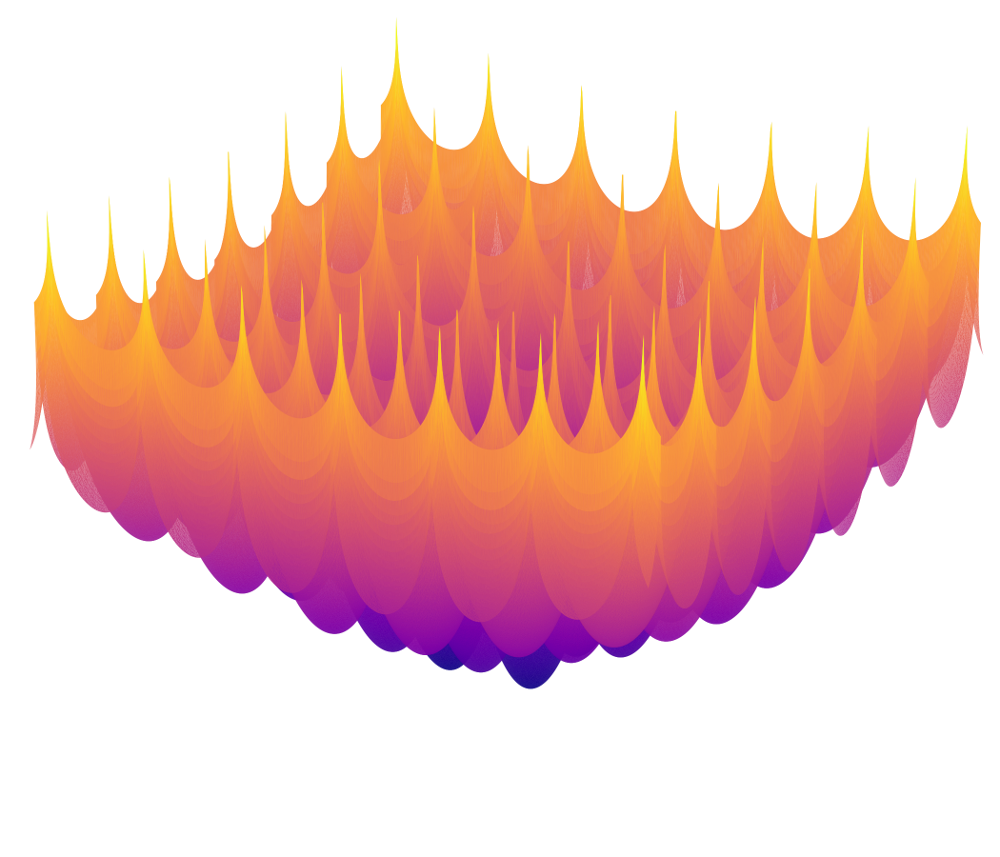
\includegraphics[width=0.195\textwidth]{robust_bo_erik/regret_plots_spiky_functions/cross_in_tray_alpha_low_res.png}
    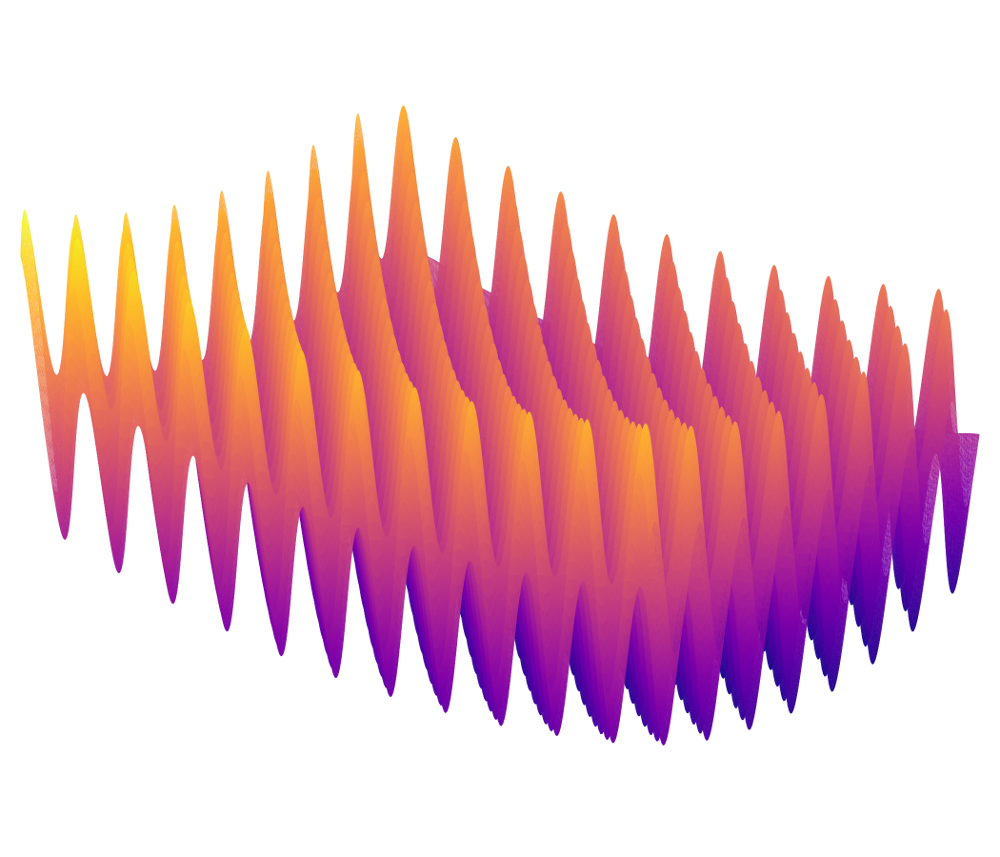
\includegraphics[width=0.195\textwidth]{robust_bo_erik/regret_plots_spiky_functions/griewank_alpha_low_res.png}
    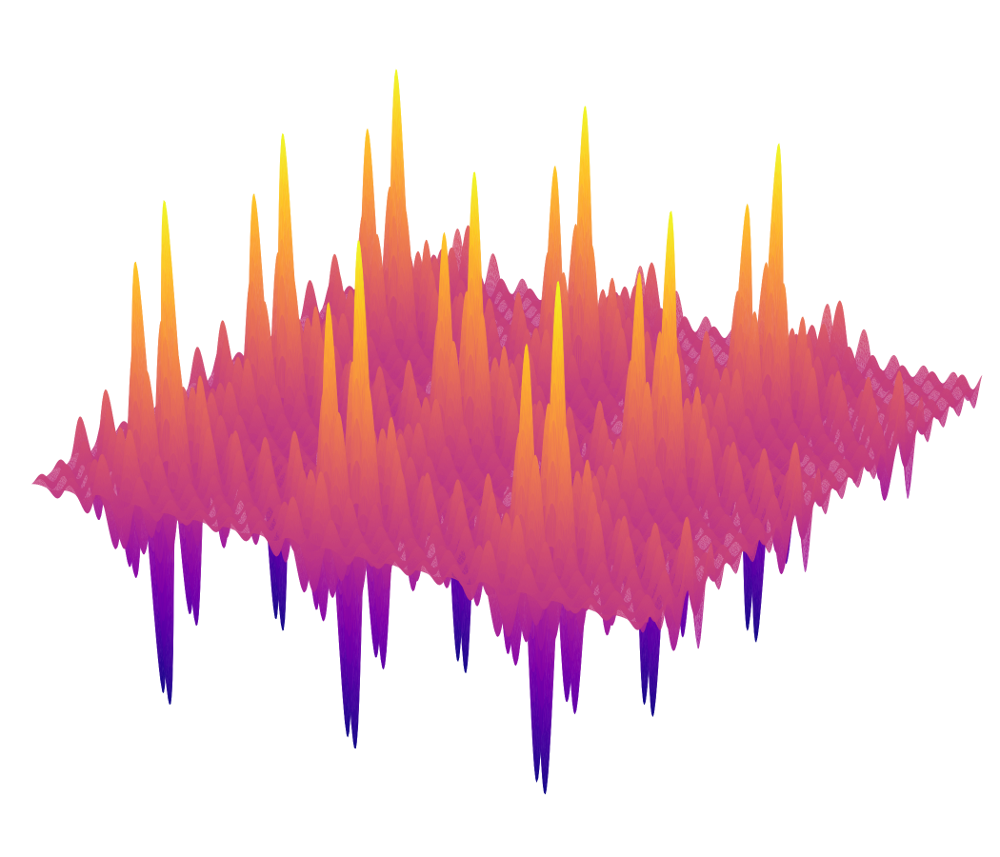
\includegraphics[width=0.195\textwidth]{robust_bo_erik/regret_plots_spiky_functions/shubert_alpha_low_res.png}
    \frame{
        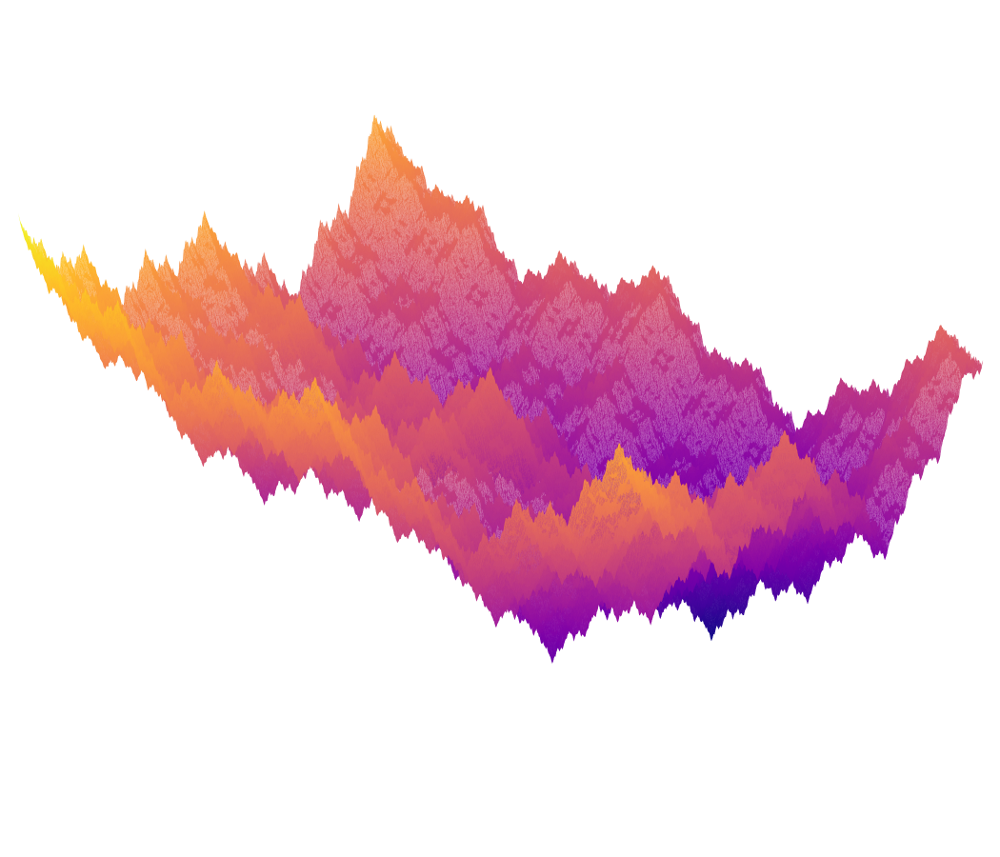
\includegraphics[width=0.195\textwidth]{robust_bo_erik/regret_plots_spiky_functions/2d_versions/weierstrass_alpha_low_res.png}
        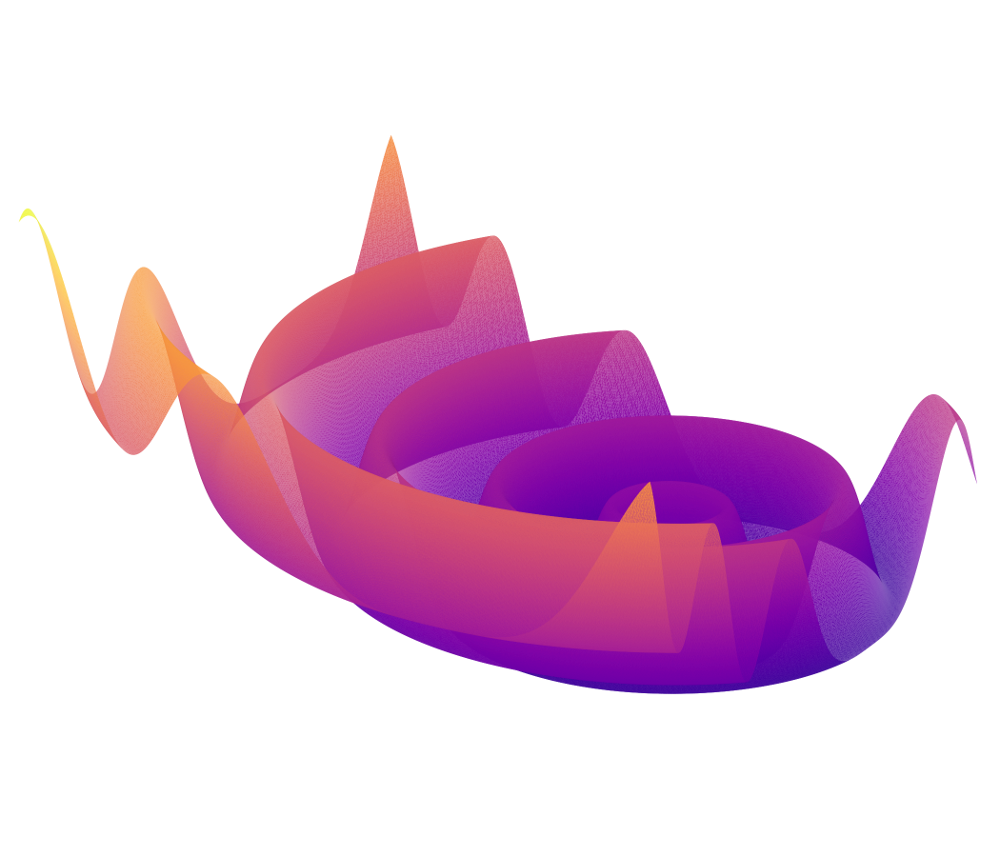
\includegraphics[width=0.195\textwidth]{robust_bo_erik/regret_plots_spiky_functions/2d_versions/deflected_corrugated_spring_alpha_low_res.png}
    }
    \caption{
        Surface plots of the benchmark functions Cross In Tray, Griewank, Shubert, Weierstrass and Deflected Corrugated Spring~\parencite{mccourt_optimization_2016}, from the left.
        The two right-most functions are available in multiple dimensionalities, where 8D and 10D is used in the experiments, respectively.
        \label{fig:bayesian_optimization:functions_plots}
    }
\end{figure}
\begin{figure}[t]
    \centering

    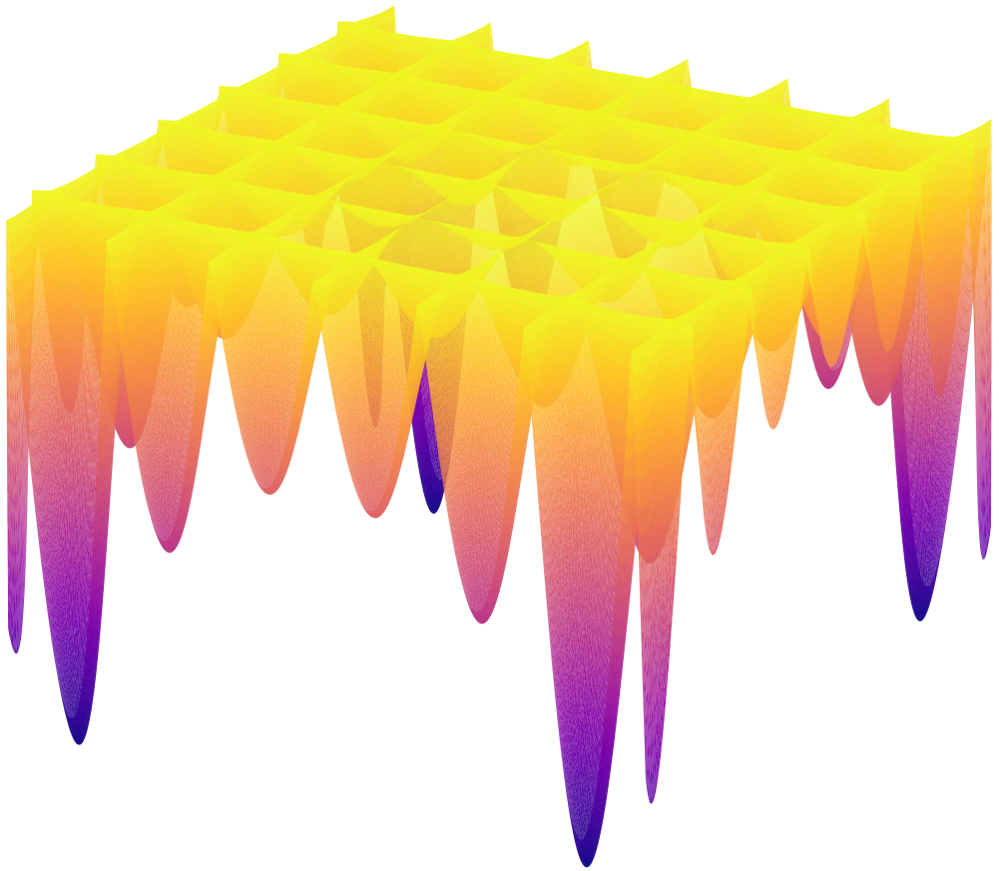
\includegraphics[width=0.235\textwidth]{robust_bo_erik/regret_plots_spiky_functions/holder_table_alpha_cropped_low_res.png}
    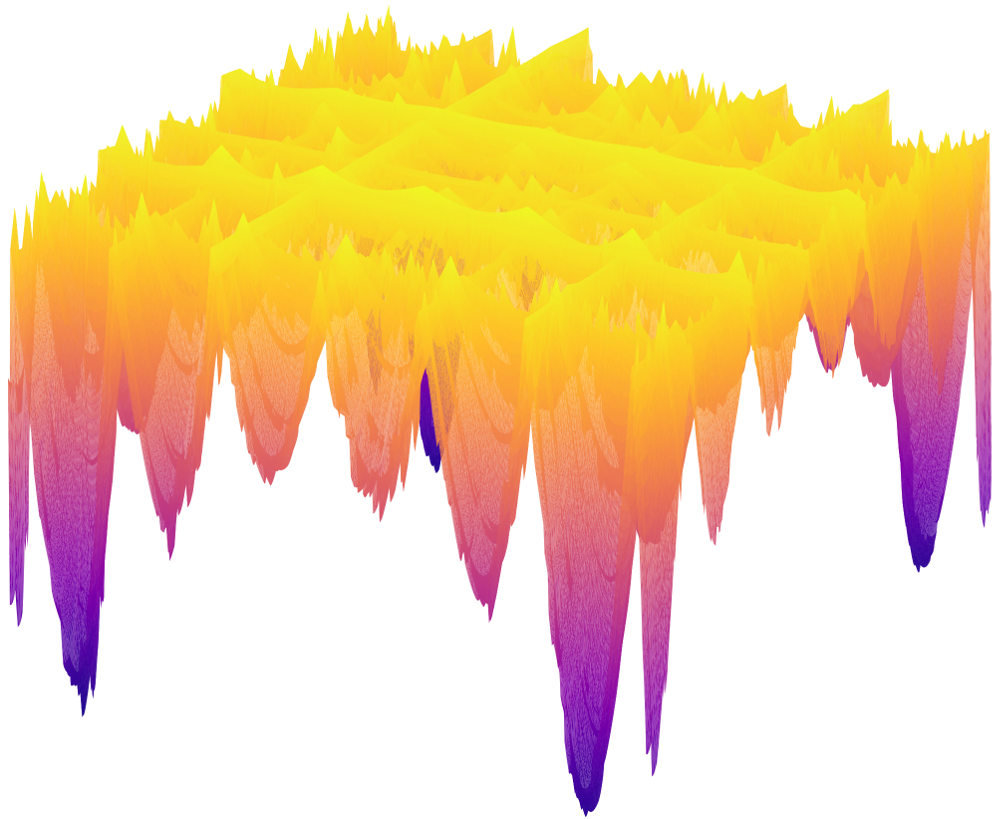
\includegraphics[width=0.235\textwidth]{robust_bo_erik/regret_plots_spiky_functions/corrupted_holder_table_alpha_cropped_low_res.png}\\
    \vspace{-2cm}
    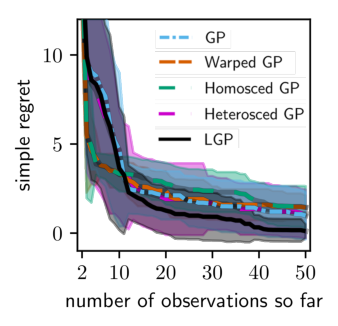
\includegraphics[width=0.235\textwidth]{robust_bo_erik/regret_plots_spiky_functions/corrupted_example/HOLDER_TABLE_2D_all_with_large_legend.pdf}
    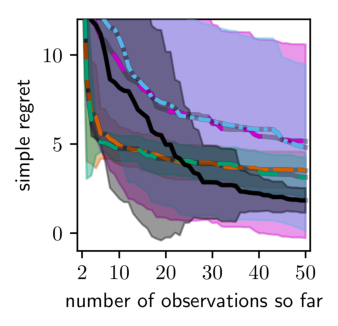
\includegraphics[width=0.235\textwidth]{robust_bo_erik/regret_plots_spiky_functions/corrupted_example/CORRUPTED_HOLDER_TABLE_2D_all_faded.pdf}
    \caption{
        A comparison of experiments on the Holder Table benchmark~\parencite{mccourt_optimization_2016} (left) and a corrupted version with added nonsmooth structure (right).
        We show plots of the respective functions and performance in terms of regret so far (over 20 repetitions).
        We show both mean regret (line) and standard deviation (shading).
        The nonsmooth structure is challenging for a noiseless GP to model and leads to a high variance in-between runs.
        Warped and homoscedasic GPs explain away the corruption, but their performance plateaus as no informative trends can be identified.
        LGP reliably identifies these trends and reliably finds good solutions.
    }

    \label{fig:bayesian_optimization:corrupted_holder}
\end{figure}

\subsection{Related Work}
\label{subsection:bayesian_optimization:related_work}
Performing BO on an objective function that is not well-behaved is very challenging.
Our method takes a Bayesian approach by incorporating a flexible noise distribution and
utilising Bayesian inference to assign the challenging details of the objective function to the noise distribution.
An alternative approach to this problem is to perform a model selection for the surrogate model, such that the choice of the surrogate model becomes a trade-off between the complexity of the model and the ability to locate the optimum under limited data, which has been explored in~\parencite{malkomes_automating_2018}.
The approach uses a compositional kernel grammar from~\parencite{duvenaud_structure_2013} to induce a space of GP models to choose from.
Although this and other model selection procedures~\parencite{malkomes_bayesian_2016,duvenaud_structure_2013,grosse_exploiting_2012,gardner_discovering_2017} themselves have shown promise,
in addition to the computational overhead, the procedures are still reliant on the existence of suitable models in this space.
It remains challenging to handle cases where the objective function contains structure that is both hard to specify a-priori, and that is unhelpful in guiding the search to the optimum.

The idea of making use of noise models for dealing with model mismatch to noise-free data is not in itself new.
In~\parencite{gramacy_cases_2010} it was shown that introducing noise in the modelling of noise-free computer experiments can lead
to models with better statistical properties such as predictive accuracy and coverage.
In that work, homoscedatic noise was addressed and used in a regression context.

In this paper we consider noise-free functions and address model misspecification of the function surrogate,
but many works have been done to make BO resilient to noisy experiments.
For example, robust noise distributions such as Student's t-distribution have been used to make BO more resilient to noise outliers~\parencite{martinez-cantin_robust_2017,martinez-cantin_practical_2017}.

Hierarchical surrogate models with input warping have been proposed to tackle BO for a non-stationary objective function~\parencite{snoek_input_2014,oh_bock_2018,calandra_manifold_2016}.
A particularly successful application is hyperparameter optimization for machine learning methods, in which the parameters are often presented in logarithmic scales.
In this case, the Beta cumulative distribution function, which only has two parameters, serves as a good warping function~\parencite{snoek_input_2014}.
Such augmentation in surrogate models requires strong domain knowledge of the objective function, and one often still has to control the increased complexity of the surrogate model, which is orthogonal to our approach.

\subsection{Experiments}

In this subsection we will demonstrate the benefit of our approach empirically.
As the approach is motivated by robustness to the presence of challenging structures in the objective function,
we will test its ability to improve search efficiency on a range of functions exhibiting such structure.
Visual examples of functions with typical properties are shown in \cref{fig:bayesian_optimization:functions_plots}.
As we will show,
our approach increases reliability in the search when faced with detrimental structure (see \cref{fig:bayesian_optimization:corrupted_holder})
that has a large negative impact on traditional surrogates.

\paragraph{Baselines and metric}
We compare with and without function modulation (\cref{toc:bayesian_optimization:modulated_objectives})
-~implemented as in \cref{toc:bayesian_optimization:latent_gp_surrogate}~-
on a popular GP model setup for BO.
In addition, we compare the LGP against other methods of handling challenging structure in the objective function,
namely (i) a noiseless GP,
(ii) a GP with homoscedastic noise,
(iii) a GP with heteroscedastic noise and
(iv) a non-stationary,
Warped GP~\parencite{snoek_input_2014}.

We follow the standard practice to compare across benchmarks and provide the \emph{mean gap} estimated over 20 runs as in~\parencite{malkomes_automating_2018}.
The gap measure is defined as $\frac{f(x_{\text{first}}) - f(x_{\text{best}})}{f(x_{\text{first}}) - f(x_{\text{optimum}})}$,
where $f(x_{\text{first}})$ is the minimum function value among the first initial random points,
$f(x_{\text{best}})$ is the best function value found within the evaluation budget and $f(x_{\text{optimum}})$ is the function's true optimum.
Methods are judged to have very similar or equivalent performance to the best performing if not significantly different,
determined by a two-sided paired Wilcoxon signed-rank test at 5\% significance~\parencite{malkomes_automating_2018}.
We also report regret (with mean and standard deviation) in the supplement.

We use the Mat\'{e}rn 5/2 kernel for all surrogates, the expected improvement acquisition function (where not otherwise stated) and Bayesian hyperparameter marginalisation as in~\parencite{snoek_practical_2012}.
For the maximization of the expected utility with respect to input location,
we use $\delta$-cover sampling, as in~\parencite{de_freitas_exponential_2012}.
The Warped GP implementation and inference is from the Spearmint package~\parencite{snoek_input_2014}.
For further details, we refer to the supplement.

\begin{table*}[t]
    \centering
    \caption{
        \label{tab:bayesian_optimization:z_table}
        Mean gap performance for various test functions; higher is better.
        The upper table shows the results after 50 objective function evaluations and the lower table after 100 evaluations.
        Due to computational cost, Warped GP results are only reported for 50 evaluations.
        Methods not significantly different from the best performing method with respect by a two-sided paired Wilcoxon signed-rank test at a 5\% significance level over 20 repetitions are shown in bold~\parencite{malkomes_automating_2018}.
        For results in terms of regret, see the supplement.
    }
    \resizebox{\textwidth}{!}{%
        \begin{tabular}{lrrlrr|rrr}
            \toprule
            {Benchmark}                    & Evals & Dim & \multicolumn{1}{c}{Properties} & \multicolumn{1}{c}{GP} & \multicolumn{1}{c}{Warped GP} & \multicolumn{1}{c}{Homosced GP} & \multicolumn{1}{c}{Heterosced GP} & \multicolumn{1}{c}{LGP} \\
            \midrule
            Hartmann                       & 50    & 6   & boring                         & \textbf{0.959}         & 0.537                         & 0.881                           & \textbf{0.973}                    & \textbf{0.937}          \\
            Griewank                       & 50    & 2   & oscillatory                    & \textbf{0.914}         & 0.493                         & 0.752                           & \textbf{0.913}                    & \textbf{0.897}          \\
            Shubert                        & 50    & 2   & oscillatory                    & 0.378                  & 0.158                         & \textbf{0.378}                  & \textbf{0.480}                    & \textbf{0.593}          \\
            Ackley $[-10, 30]^d$           & 50    & 2   & complicated, oscillatory       & \textbf{0.924}         & 0.274                         & \textbf{0.892}                  & \textbf{0.912}                    & \textbf{0.927}          \\
            Cross In Tray                  & 50    & 2   & complicated, oscillatory       & \textbf{0.954}         & 0.385                         & 0.929                           & \textbf{0.977}                    & \textbf{0.945}          \\
            Holder table                   & 50    & 2   & complicated, oscillatory       & 0.939                  & 0.896                         & 0.900                           & 0.931                             & \textbf{0.993}          \\
            Corrupted Holder Table         & 50    & 2   & complicated, oscillatory       & 0.741                  & 0.798                         & 0.826                           & 0.729                             & \textbf{0.896}          \\
            \midrule
            Branin01                       & 100   & 2   & none                           & \textbf{1.000}         &                               & \textbf{1.000}                  & \textbf{1.000}                    & \textbf{1.000}          \\
            Branin02                       & 100   & 2   & none                           & \textbf{0.991}         &                               & 0.964                           & \textbf{0.990}                    & \textbf{0.981}          \\
            Beale                          & 100   & 2   & boring                         & \textbf{0.987}         &                               & \textbf{0.982}                  & \textbf{0.987}                    & \textbf{0.988}          \\
            Hartmann                       & 100   & 6   & boring                         & \textbf{0.987}         &                               & 0.947                           & \textbf{0.984}                    & \textbf{0.979}          \\
            Griewank                       & 100   & 2   & oscillatory                    & \textbf{0.967}         &                               & 0.875                           & \textbf{0.969}                    & \textbf{0.946}          \\
            Levy                           & 100   & 2   & oscillatory                    & \textbf{0.997}         &                               & \textbf{0.999}                  & \textbf{0.998}                    & \textbf{0.998}          \\
            Deflected Corrugated Spring    & 100   & 10  & oscillatory                    & 0.347                  &                               & \textbf{0.840}                  & 0.406                             & 0.697                   \\
            Shubert $[-10, 10]^d$          & 100   & 2   & oscillatory                    & 0.510                  &                               & 0.511                           & \textbf{0.672}                    & \textbf{0.877}          \\
            Weierstrass                    & 100   & 8   & complicated                    & 0.600                  &                               & \textbf{0.704}                  & 0.577                             & 0.625                   \\
            Cross In Tray                  & 100   & 2   & complicated, oscillatory       & \textbf{1.000}         &                               & 0.995                           & \textbf{1.000}                    & \textbf{1.000}          \\
            Holder Table                   & 100   & 2   & complicated, oscillatory       & 0.971                  &                               & 0.963                           & \textbf{0.964}                    & \textbf{1.000}          \\
            Ackley $[-10, 30]^d$           & 100   & 2   & complicated, oscillatory       & \textbf{0.971}         &                               & 0.914                           & \textbf{0.980}                    & \textbf{0.974}          \\
            Ackley $[-10, 30]^d$           & 100   & 6   & complicated, oscillatory       & 0.459                  &                               & \textbf{0.789}                  & 0.442                             & \textbf{0.712}          \\
            Corrupted Holder Table         & 100   & 2   & complicated, oscillatory       & 0.844                  &                               & 0.889                           & 0.822                             & \textbf{0.918}          \\
            Corrupted Exponential          & 100   & 8   & complicated, oscillatory       & 0.580                  &                               & \textbf{0.847}                  & 0.581                             & \textbf{0.806}          \\
            \midrule
            HPO: NN Boston                 & 100   & 9   & unknown                        & \textbf{0.720}         &                               & \textbf{0.761}                  & \textbf{0.810}                    & \textbf{0.770}          \\
            HPO: NN Climate Model Crashes  & 100   & 9   & unknown                        & 0.629                  &                               & \textbf{0.717}                  & \textbf{0.683}                    & \textbf{0.678}          \\
            Active learning: Robot Pushing & 100   & 4   & unknown                        & 0.877                  &                               & 0.745                           & \textbf{0.907}                    & \textbf{0.932}          \\
            \bottomrule
        \end{tabular}
    }
    \medskip
\end{table*}

\begin{figure}[t]
    \centering
    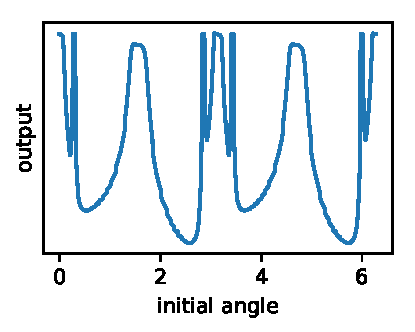
\includegraphics[width=0.31\textwidth]{robust_bo_erik/robot_pushing/robot_pushing_initial_angle.pdf}
    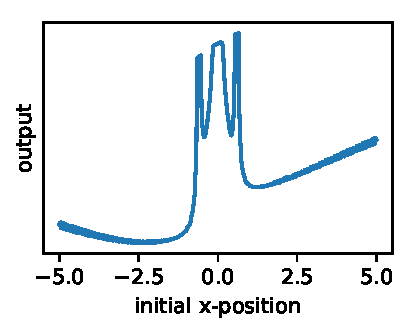
\includegraphics[width=0.31\textwidth]{robust_bo_erik/robot_pushing/robot_pushing_x_position.pdf}
    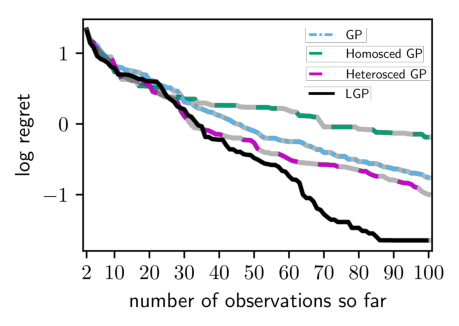
\includegraphics[width=0.335\textwidth]{robust_bo_erik/robot_pushing/robot_pushing_with_legend.pdf}
    %    
\includegraphics[width=0.45\textwidth]{robust_bo_erik/real_world/legend.pdf}\\
    %    \vspace{-0.3cm}
    \caption{
        Active learning: Robot pushing.
        The objective function to be optimized takes as input the pushing action of a robot within a simulation,
        and outputs the distance of the pushed object to the goal location.
        The two plots on the left show that the task surface, resulting from the dynamic system, is nonsmooth and non-trivial.
        The right plot shows the mean regret and standard deviations for the different surrogates.
        As can be seen, the LGP found good solutions with low variance, improving reliability of the search.
        The 1D slices of the 4D function (the two from the left) was generated by fixing the initial y-position (param.) to the one of the goal position,
        the simulation steps (param.) to the center of its domain, and varying the initial angle (param.) or the x-position (param.), respectively,
        while keeping the other fixed at zero.
        Slicing the 4D function differently produced similar nonsmooth response curves.\\
        \label{fig:bayesian_optimization:real_world}
    }
\end{figure}

\paragraph{Benchmark datasets}
We perform the comparisons on benchmarks from~\parencite{mccourt_optimization_2016,head_scikit-optimize_2018} using the default domains provided by respective benchmark, detailed in the supplement.
%Some problems are available in different dimensionalities, which are denoted in with the results.
%We note that in experiments in other work, domains are sometimes restricted, which changes the characteristics and difficulty of the benchmark problem.
In addition, problems are marked with the descriptive properties given in~\parencite{mccourt_optimization_2016} and in the supplement that can reflect the relative difficulty of the task.

\paragraph{Priors on the latent input variables}
The prior $\Prob{\mat{h}_n} = \Gaussian{\mat{0}, \sigma_h^2\mathbb{I}}$ can be parameterized in relation to the relative scale of the characteristics to be ignored.
We specify the function prior over the product space $\Xc \times \Zc$ using a kernel with common parameters for $\mat{x}_n$ and $\mat{h}_n$.
Thus, the standard deviation of the prior $\sigma_h$ relates directly to distances in the $\Xc$-direction.
When domain-specific knowledge is available, $\Prob{\mat{H}}$ may be specified at an appropriate scale.
However, we often do not have access to such knowledge.
In all our experiments, we adopt a hierarchical prior approach whereby $\sigma_h$ is sampled uniformly from a small candidate set at each evaluation.
Specifically, $\sigma_h \sim \Uniform{\Set{0.1 d, 0.01 d, 0}}$ where $d = \sqrt{Q}$, the length of the diagonal of the unit Q-dimensional hypercube.
We found that this approach performed well empirically and is applied consistently across all our experiments where not otherwise specified.
A choice of $\sigma_h \to 0$ corresponds to a noiseless GP without latent covariates.

\paragraph{Evaluation on benchmark suite}
\Cref{tab:bayesian_optimization:z_table} presents results across a wide range of benchmark functions consisting of the SigOpt benchmark suite~\parencite{mccourt_optimization_2016}.
Three additional real-world benchmarks~\parencite{head_scikit-optimize_2018,malkomes_automating_2018,kaelbling_learning_2017} are included in the bottom subsection of the table.
The benchmarks from~\parencite{mccourt_optimization_2016} are popular functions used in both black-box optimization as well as classic optimization literature.
As of the focus of the paper, benchmarks from the literature exhibiting challenging properties such as oscillatory local structures were included,
in addition to simpler functions for reference.

In general, the noise-free, homoscedastic and heteroscedastic noise GPs tend to either share best place with the LGP or be outperformed by
it.
The Warped GP, which warps the input space to obtain a tight fit to the data, consistently struggle with the complicated and oscillatory benchmarks.
On some benchmarks there are large differences in favour of using noisy surrogates on the noise-free benchmarks.
Such an example is Ackley 6D, which in the dataset is described as \enquote{technically oscillatory, but with such a short wavelength that its behavior probably seems more like noise}~\parencite{mccourt_optimization_2016}.
Another example is the Shubert function, which has multiple sharp local optima surrounded by large oscillations.
On 2 of 18 benchmarks, the LGP was not best (or within the two-sided Wilcoxon test), but instead the homoscedastic GP.
These functions were Weierstrass, which has a homoscedastic characteristic (see \cref{fig:bayesian_optimization:functions_plots}),
and Deflected Corrugated Spring, on both of which the LGP obtained the second highest mean gap.
In contrast to the LGP and the heteroscedastic GP, the noise model of the homoscedastic GP sometimes hurt performance in relation to the noise-free GP.
Given the black-box nature of functions in BO, it is important that the surrogate noise model 'turns off' adequately when not needed.
The heteroscedastic GP provided significant benefit on two benchmarks over the GP,
whereas the LGP provided such benefit on \emph{eight} benchmarks.

\paragraph{Real-world} Apart from widely used synthetic functions,
we also compare our method on three real-world problems.
The results are shown in the last three rows of \cref{tab:bayesian_optimization:z_table}.
One of the benchmarks is an active learning task of a robot pushing a box within a simulation.
As we show in \cref{fig:bayesian_optimization:real_world}, the benchmark's response surface is both nonsmooth and oscillatory.
The LGP reliably found good solutions on the benchmark, while the other surrogates sometimes failed, resulting in high variances.
The homoscedastic GP performed the worst,
which we suspect is due to the nonsmooth and heavily oscillatory structures forces a high global noise level,
which may lead to failure in utilising informative structure in other regions.

\paragraph{Other aquisition functions} We suggest that the problem with structures challenging to model is relevant to address irrespective of the acquisition function.
To confirm that the method is applicable also using other acquisition functions we ran the Corrupted Exponential benchmark
using both Expected Improvement (EI) and Lower Confidence Bound (LCB) with the default exploration weight ($=2.0$) from GPyOpt~\parencite{gpyopt_gpyopt_2016}.
As can be seen in \cref{tab:bayesian_optimization:z_table}, in the case of EI, the GP and the heteroscedastic GP performed worse than the homoscedastic GP and the LGP.
The homoscedastic GP achieved the highest mean gap, but the difference was not significant under the Wilcoxon test to the LGP which obtained a similar mean gap.
Using the LCB acquisition function the performance for the homescedastic GP decreased to $0.818$ and the LGP increased to $0.858$,
and their difference in rank in favour of the LGP was significant under the test.
The heteroscedastic GP increased using LCB to $0.797$ and the GP to $0.751$, remaining as worst performing.

As the experimental evaluation demonstrates,
our suggested approach for handling challenging structures in the objective function consistently improved reliability and performance
over the traditional surrogate on a wide range of benchmarks.
Importantly, on benchmarks where the extended methodology were not needed the performance aligned with that of the traditional surrogate.
When it was needed, it was shown to often have a large positive impact on overall efficiency of the search.

\subsection{Conclusion}
We have presented an approach to Bayesian Optimization where the surrogate model is alleviated from needing to explain the observed objective function values perfectly,
which is challenging for complicated or nonsmooth functions.
Instead, we model the essential structure of the objective function that is well-behaved and leave the rest of the function details to be absorbed in a noise distribution.
We show experimentally how our approach is able to solve synthetic and real-world benchmarks with challenging local structures reliably.
Importantly our methodology can be applied to any surrogate model used for BO,
and the specific case addressed in the paper can be included in any Gaussian process-based surrogate.


\section{Reinforcement Learning}
\label{toc:bayesian_rl}
\parencite{bertsekas_stochastic_1978}

\begin{definition}[Reinforcement Learning Problem]
    An \emph{infinite horizon stochastic reinforcement learning problem} is a tuple $(\Sc, \Ac, \Zc, \Prob{z \given s, a}, f, \gamma, r)$ consisting of
    \begin{labeling}{Disturbance kernel $\Prob{z \given s, a}$\quad}
        \item[State space $\Sc$] A nonempty measurable space;
        \item[Action space $\Ac$] A nonempty measurable space;
        \item[Disturbance space $\Zc$] A nonempty measurable space;
        \item[Disturbance kernel $\Prob{z \given s, a}$] A measurable function in $\Sc \times \Ac \to \Probs{\Zc}$;
        \item[System function $f$] A measurable function in  $\Sc \times \Ac \times \Zc \to \Sc$;
        \item[Discount factor $\gamma$] A positive real number;
        \item[Reward function $r$] A differentiable function in $\Sc \times \Ac \to \Rb \cup \Set{\pm \infty}$.
    \end{labeling}
\end{definition}
We remove the control constraint because nobody cares.


\subsection{Reinforcement Learning}
\label{toc:bayesian_rl:bayesian_rl}
\begin{figure}[t]
    \centering
    \includestandalone{figures/agent_environment_interaction}
    \caption[Agent-environment interaction]{
        The interaction between an agent and its environment in reinforcement learning happens at discrete time steps.
    }
    \label{fig:bayesian_rl:agent_environment_interaction}
\end{figure}
Reinforcement learning describes the general problem of learning to control a system by interaction in order to achieve a predefined goal.
An \emph{agent} has to decide on specific \emph{actions} to influence their \emph{environment}.
The boundary between agent and environment is shown in \cref{fig:reinforcement_learning:agent_environment_interaction}.
They interact at specific discrete \emph{time steps} $t \in \Nb$.
At every such time step, the agent observes the environment via the \emph{state} $\mat{s}_t \in \Sc$, where $\Sc$ is the space of all possible states.
Based on this information, the agent has to decide which action $\mat{a}_t \in \Ac$ to perform.
The space of all possible actions $\Ac$ is assumed to be constant for all time steps and states.
The decision-process an agent employs in order to choose an action is called the agent's \emph{policy}.

\begin{definition}[Policy]
    A \emph{policy $\pi$} an agent follows encodes the choice it makes when faced with a decision.
    It is a function
    \begin{align}
        \pi: \Sc \to \Ac
    \end{align}
    which maps the current state of the system to the action the agent will perform.
\end{definition}

Once the agent has chosen an action for time step $t$, the state $\mat{s}_{t+1}$ is generated by the \emph{transition dynamics} $f$.
These dynamics are unknown to the agent and can contain probabilistic components such as noise.
However, the agent always observes one realization $\mat{s}_{t+1}$, the actual next state of the system.
This implies that given the same initial state $\mat{s}_0$ and policy $\pi$ it might be possible to generate different \emph{trajectories} $(\mat{s}_0, \dots, \mat{s}_T)$ by applying the transition dynamics $T$ times.
Together with the state and action spaces, the transition dynamics fulfill the Markov property.
That is, the distribution of $\mat{s}_{t+1}$ is independent of all states before $\mat{s}_t$ given $\mat{s}_t$.
\begin{definition}[Transition Dynamics]
    \label{def:bayesian_rl:transition_dynamics}
    The \emph{transition dynamics $f$} of a system encode its physical behaviour.
    These dynamics
    \begin{align}
        f: \Sc \times \Ac \to \Sc
    \end{align}
    stay constant over time but can be probabilistic.
\end{definition}

At time step $t+1$, the agent observes the state $\mat{s}_{t+1}$.
Additionally, it also receives a \emph{reward $r_{t+1}$}.
The reward is a quality assigned to the state transition from $\mat{s}_t$ to $\mat{s}_{t+1}$ using the action $\mat{a}_t$.
The higher the reward, the better the state transition is considered to be, independently of the future or past development of the system.
In the following, we consider $r_{t+1}$ to be independent of the state $\mat{s}_t$ and the action $\mat{a}_t$ and only depend on $\mat{s}_{t+1}$.
It is obtained from a real-valued and known \emph{reward function $r$} such that $r_{t+1} = r(\mat{s}_{t+1})$.
\begin{definition}[Reward Function]
    \label{def:bayesian_rl:reward_function}
    The \emph{reward function $r$} assigns a quality to each state in the state space
    \begin{align}
        r : \Sc \to \Rb.
    \end{align}
    This reward is the immediate feedback an agent receives when interacting with the system.
\end{definition}

The goal of the agent is to maximize the sum of all rewards earned while interacting with the system.
A greedy agent which is only concerned with the next immediate reward might not be the most successful, since it may be necessary to make a decision which is bad in the short term to gain an advantage in the long run, such as sacrificing a piece in chess to end up in a better position overall.

The \emph{value function} is a measure for how good a policy behaves in the long run.
Given a policy and an initial state, it is defined as the expected sum of rewards earned in a time horizon $T$.
Since the transition dynamics are assumed to be probabilistic, the states at all time steps greater than zero can be random variables.
Given a distribution of the state $\mat{s_t}$, the distribution for the next state $\mat{s_{t+1}}$ is
\begin{align}
    \Prob{\mat{s_{t+1}}} & = \int \Fun{f}{\mat{s_{t+1}} \given \mat{s_t}, \pi}\Prob{\mat{s_t}} \diff \mat{s_t},
\end{align}
where $f\Cond{\mat{s_{t+1}} \given \mat{s_t}, \pi(\mat{s_t})}$ denotes the probability of $\mat{s_{t+1}}$ under the distribution $f(\mat{s_t}, \pi(\mat{s_t}))$.

The time horizon $T$ can be chosen freely but does not depend on the policy or state.
The larger the time horizon, the more far-sighted an agent has to be to be successful.
For large values of $T$, it can be helpful to focus on rewards earned in the near future and to weight potential rewards further along with a smaller factor.
This is achieved with a constant discount factor $\gamma$.
\begin{definition}[Value Function]
    \label{def:bayesian_rl:old_value_function}
    Given transition dynamics $f$, a policy $\pi$, a time horizon $T \in \Nb \cup \left\{ \infty \right\}$ and a discount factor $0 \leq \gamma \leq 1$, the \emph{(expected) value function $J^\pi$} denotes the expected accumulated reward of a state and is given by
    \begin{align}
        J^\pi : \left\{
        \begin{aligned}
            \Sc     & \to \Rb                                                                                      \\
            \mat{s} & \mapsto \Moment*{\E}{\sum_{t=1}^T \gamma^t r(\mat{s}_t) \given f, \pi, \mat{s}_t = \mat{s}}.
        \end{aligned}
        \right.
    \end{align}
    If the time horizon is infinite, $\gamma$ must be smaller than 1.
\end{definition}

Given a distribution of possible initial states $\Prob{\mat{s}_0}$, the sets $\Sc$ and $\Ac$ of states and actions together with the transition dynamics $f$, and the reward function $r$, reinforcement learning can be interpreted as a fully observable Markov decision process (MDP).
Note that extensions to partially observable MDPs (POMDPs) are regularly considered in the RL setting.

The objective of the reinforcement learning problem is to find the best policy in this decision process under the assumption that the transition dynamics are unknown a priori.
The \emph{optimal policy} $\pi^*$ maximizes the expected value under the distribution of initial states, that is it solves the optimization problem
\begin{align}
    \label{eq:bayesian_rl:optimal_policy}
    \begin{split}
        \pi^\ast &\in \argmax_{\pi} \Moment*{\E_{\Prob{\mat{s}_0}}}{J^\pi(\mat{s}_0)} \\
        &= \argmax_{\pi} \int J^\pi(\mat{s}_0) \Prob{\mat{s}_0} \diff \mat{s}_0.
    \end{split}
\end{align}


\subsection{Probabilistic Reinforcement Learning}
\label{toc:bayesian_rl:probabilistic_reinforcement_learning}
\begin{figure}[t]
    \centering
    \includestandalone{figures/quantities_of_interest_rl}
    \caption[Quantities of interest in reinforcement learning]{
        Quantities of interest in reinforcement learning.
        \label{fig:bayesian_rl:quantities_of_interest_rl}
    }
\end{figure}
\begin{table}[t]
    \centering
    \caption{Great Table!}
    \label{tab:bayesian_rl:label}
    \newcolumntype{Y}{>{\centering\arraybackslash}X}
    \begin{tabularx}{\textwidth}{cYY}
        \toprule
                          & Probabilistic Numerics & Reinforcement Learning \\
        \midrule
        $\Uc$             & Latent function        & True system-dynamics   \\
        $\Qc$             & Definite Integral      & Optimal value          \\
        $\Yc$             & Function evaluations   & Batch/Online data      \\
        \midrule
        $Q : \Uc \to \Qc$ & Integration            & Bellman principle      \\
        $Y : \Uc \to \Yc$ & Observation            & Exploration            \\
        $B : \Yc \to \Qc$ & Quadrature             & Policy search          \\
        \bottomrule
    \end{tabularx}
\end{table}


\subsection{Bayesian Reinforcement Learning}
\label{toc:bayesian_rl:bayesian_reinforcement_learning}
?
